\documentclass[review]{elsarticle}

\usepackage{graphics, float, url}
\usepackage{graphicx}
\usepackage{subcaption}
\usepackage{lineno,hyperref}
\usepackage{mathtools}
\usepackage{multirow}
\usepackage{adjustbox}
\usepackage{chngpage}
\usepackage{setspace}
\usepackage{amsfonts}
\usepackage{subcaption}
\usepackage{float}
\usepackage[ruled, lined, onelanguage, linesnumbered]{algorithm2e}
\usepackage[usenames,dvipsnames,svgnames,table]{xcolor}
\newcommand{\myfloatalign}{\centering}
\modulolinenumbers[5]

\usepackage{epstopdf}
\epstopdfDeclareGraphicsRule{.tiff}{png}{.png}{convert #1 \OutputFile}
\AppendGraphicsExtensions{.tiff}

\journal{Applied Soft Computing}

%%%%%%%%%%%%%%%%%%%%%%%
%% Elsevier bibliography styles
%%%%%%%%%%%%%%%%%%%%%%%
%% To change the style, put a % in front of the second line of the current style and
%% remove the % from the second line of the style you would like to use.
%%%%%%%%%%%%%%%%%%%%%%%

%% Numbered
%\bibliographystyle{model1-num-names}

%% Numbered without titles
%\bibliographystyle{model1a-num-names}

%% Harvard
%\bibliographystyle{model2-names.bst}\biboptions{authoryear}

%% Vancouver numbered
%\usepackage{numcompress}\bibliographystyle{model3-num-names}

%% Vancouver name/year
%\usepackage{numcompress}\bibliographystyle{model4-names}\biboptions{authoryear}

%% APA style
%\bibliographystyle{model5-names}\biboptions{authoryear}

%% AMA style
%\usepackage{numcompress}\bibliographystyle{model6-num-names}

%% `Elsevier LaTeX' style
\bibliographystyle{elsarticle-num}
%%%%%%%%%%%%%%%%%%%%%%%
\newtheorem{definition}{Definition}
\begin{document}

\begin{frontmatter}

\title{Enhancing instance-level constrained clustering through differential evolution}

\author[mymainaddress]{Germ\'an Gonz\'alez-Almagro\corref{mycorrespondingauthor}}
\cortext[mycorrespondingauthor]{Corresponding author}
\ead{germangalmagro@ugr.es}

\author[mymainaddress]{Juli\'an Luengo}

\author[mysecondaddress]{Jos\'e-Ram\'on Cano}

\author[mymainaddress]{Salvador Garc\'ia}

\address[mymainaddress]{DaSCI Andalusian Institute of Data Science and Computational Intelligence, University of Granada, Spain}

\address[mysecondaddress]{Dept. of Computer Science, EPS of Linares, University of Ja\'en, Campus Cient\'ifico Tecnol\'ogico de Linares, Cintur\'on Sur S/N, Linares 23700, Ja\'en, Spain}

\begin{abstract}
This paper proposes an adaptation of the successful SHADE method to solve the constrained clustering problem. This problem consists of a modification of the traditional clustering to consider a new type of information, which is given in the form of must-link and cannot-link constraints. We will compare the results obtained on 25 datasets by this new SHADE adaptation with a previous heuristic-based approach---BRKGA---as well as with some of the state-of-the-art-methods, supporting our conclusions with the aid of Bayesian tests.
\end{abstract}

\begin{keyword}
constrained clustering, must-link, cannot-link, genetic algorithm, differential evolution.
\end{keyword}

\end{frontmatter}

\linenumbers

\section{Introduction} \label{sec:Intro}

One of the most widely known and studied data analysis problems is clustering. It is one of the most successful methods in the field of unsupervised learning, where there is no supervision on how the information should be handled. Clustering has been able to provide solutions in a large number of knowledge fields, such as, marketing, banking, psychology, psychiatry, astronomy, archaeology and genetics among others \cite{ClusterAnalysis}.

In the literature, clustering methods are often divided into two subsets: partitional clustering and hierarchical clustering. The main difference is that in hierarchical clustering the result is not a partition of the data with a certain number of clusters---as in partitional clustering---, but instead a dendrogram in which there are partitions that include from the whole dataset to particular individuals \cite{ClusterAnalysis}. In this paper we will focus on partitional clustering. \textcolor{red}{Poner ejemplos de cada uno (con referencias)?}

We can define partitional clustering as the task of grouping the instances of a dataset into $k$ clusters, so that new information can be extracted from them. A dataset $X$ is composed of $n$ instances, each one of them described by $d$ features. More formally, $X = \{x_1, \cdots, x_n\}$, with the $i$th instance noted as $x_i = (x_{[i,1]}, \cdots, x_{[i,d]})$. A typical clustering algorithm assigns a class label $l_i$ to each instance $x_i \in X$. As a result, we obtain the set of labels $L = \{l_1, \cdots, l_n\}$, with $l_i \in \{1, \cdots, k\}$, that effectively splits $X$ into $k$ non-overlapping clusters $c_i$ to form a partition called $C$. The criterion used to assign an instance to a given cluster is the similarity to the rest of elements in that cluster, and the dissimilarity to the rest of instances of the dataset, which can be obtained with some kind of distance measurement $d(\cdot, \cdot)$. An important detail is that each instance must belong to a single cluster. \cite{jain1999data}

\textcolor{red}{Bucar una referencia fiable de ssl}

Constrained clustering is a semi-supervised learning method. Its goal is to find a partition of the dataset that meets the proper characteristics of a clustering method result, in addition to satisfying a certain constraint set. It has been succesfully applied in many knowledge fields. It has been used to guide the movement of walking robots, as well as in other advanced robotics applications \cite{davidson2005clustering, semnani2016constrained}. In \cite{seret2014new} constrained clustering is presented as a useful tool in the context of applied marketing. Biology has also made use of constrained clustering, being able to detect simultaneous appearances of genes and proteins in biological data bases \cite{segal2003discovering}. In \cite{levy2008structural} a method of segmenting musical audio into separated sections using constrained clustering is described. Constrained clustering has also been useful to classify Internet traffic, which is considered to be one of the most fundamental functionalities in the network management field \cite{wang2014internet}. Electoral district design problems can also be approached using constrained clustering, as shown in \cite{brieden2017constrained}. Lastly, it is mandatory to name the widely known application to GPS data of constrained clustering, presented in \cite{wagstaff2001constrained}.

Constraints can be understood in different ways, resulting in three main types of constrained clustering: cluster-level, instance-level and feature-level constrained clustering \cite{bradley2000constrained,davidson2007survey,schmidt2011clustering}. Moreover, hybrid approaches which try to integrate different types of constraints have also been proposed \cite{wang2010clustering}. 

In particular, we can find in the literature two types of instance-level constraints: pairwise constraints and distance-based constraints. Pairwise constraints tell us if two specific instances of a dataset must be placed in the same or in different clusters, resulting in Must-link (ML) and Cannot-link (CL) constraints respectively. On the other hand, distance-based constraints do not involve specific instances, but tell us if instances must be placed in the same or in different clusters based on a given distance measure.\cite{davidson2007survey} This paper focuses on pairwise instance-level constraints (ML and CL), which will be discussed later in Section \textcolor{red}{X}.

Regarding the degree to which the constraints have to be satisfied, we can make a distinction between the concepts of hard and soft constraints. Hard constraints must necessarily be satisfied in the output partition of any algorithm that makes use of them, while soft constraints are taken as a strong guide for the algorithm that uses them but can be partially satisfied in the output partition \cite{seret2014new, wagstaff2001constrained, law2004clustering}. For the purposes of this paper, we will employ the latter.

Finding the optimal partition in a dataset, with respect to any kind of reasonable criteria, is known to be a $\mathbf{NP}$-hard problem. Therefore, the incorporation of constraints may modify the complexity of the clustering problem, depending on the type of constraints used. As we will study in more depth in Section \ref{sec:BackFeas}, the use of ML and CL constraints makes the constrained clustering problem $\mathbf{NP}$-complete. \cite{davidson2005clustering}

The constrained clustering problem can be formulated in terms of optimization, so that we can apply various optimization techniques to solve it. As mentioned earlier, it is a difficult problem to solve, so nature-inspired techniques are presented as a promising option to find quality approximate solutions. Nature is the best example of adaptive problem solving since it can apply an optimal strategy suited for each natural phenomenon \cite{fausto2019ants}. Nature-inspired algorithms are designed to emulate natural optimization phenomena, such as evolution, collective behavior of animals, physics laws or even human being-related processes. There have been attempts to solve the constrained clustering problem with nature-inspired algorithms, such as the adaptation of the Biased Random-key Genetic Algorithm (BRKGA), which can be found in \cite{de2017comparison}. Swarm-based methods have also been applied to constrained clustering, such as the one presented in \cite{xu2013improving}.

Differential Evolution (DE) is an evolution-based algorithm that has proven to be excellent in real-domain problem solving \cite{das2011differential}; in this paper we propose a new DE variant to find quality solutions for the constrained clustering problem (see Section \ref{sec:SHADE}). We will make use of the Random-key concept from BRKGA, along with proposing a new fitness function, to build the already mentioned DE variant. We will properly compare the results obtained by our new method with previous nature-inspired algorithms, as well as with the constrained clustering state-of-the-art.

\textcolor{red}{Cambiar el parrafo de abajo en funcion de como quede la organizacion de secciones final}

Regarding the organization of this paper, Section \ref{sec:background} reviews the existing knowledge concerning constrained clustering and DE. In Section \ref{sec:brkga} we will briefly review the BRKGA algorithm and its adaptation for constrained clustering. Afterward, a variant of DE algorithm will be presented in Section \ref{sec:SHADE}, followed by its adaptation for constrained clustering and a new fitness function. Sections \ref{sec:expSetup} to \ref{sec:analisis} present the experimental setup, results and their analysis. Finally, in Section \ref{sec:conclusiones} we discuss conclusions.

\section{Background} \label{sec:background}

In this section we present the background knowledge concerning constrained clustering (Section \ref{sec:BackCC}), its computational complexity (Section \ref{sec:BackFeas}) and a brief description of some of the state-of-the-art methods for constrained clustering \ref{sec:BackSOTA}. We will also present the basis of the DE optimization method (Section \ref{sec:BackDE}).

\subsection{Constrained Clustering} \label{sec:BackCC}

In most clustering applications it is common to have some kind of information about the dataset to be analyzed. In pairwise instance-level constrained clustering this information is given in the form of pairs of instances. A constraint states whether the instances which it refers to must, or must not, be assigned to the same cluster. It is possible to obtain a better result by using this type of information than by using completely unsupervised clustering algorithms.

Given the notation for the clustering problem introduced in Section \ref{sec:Intro}, we can now formalize the two type of constraints mentioned: 

\begin{itemize}

	\item Must-link constraints $C_=(x_j,x_i)$: instances $x_i$ and $x_j$ from $X$ must be placed in the same cluster.

	\item Cannot-link constraints $C_{\neq}(x_i,x_j)$: instances $x_i$ and $x_j$ from $X$ cannot be assigned to the same cluster.

\end{itemize}

The goal of constrained clustering is to find a partition (or clustering) of $k$ clusters $C = \{c_1, \cdots, c_k\}$ of the dataset $X$ that ideally satisfies all constraints in the constraint set. As in the original clustering problem, it must be fulfilled that the sum of instances in each cluster $c_i$ is equal to the number of instances in $X$, which we have defined as $n = |X| = \sum_{i = 1}^{k} |c_i|$.

Knowing how a constraint is defined, ML constraints are an example of an equivalence relation; therefore, ML constraints are reflexive, transitive and symmetric. This way, given constraints $C_=(x_a,x_b)$ and $C_=(x_b,x_c)$ then $C_=(x_a,x_c)$ is verified. In addition, if $x_a \in c_i$ and $x_b \in c_j$ are related by $C_=(x_a,x_b)$, then $C_=(x_c,x_d)$ is verified for any $x_c \in c_i$ and $x_d \in c_j$ \cite{xu2013improving}\cite{davidson2007survey}.

On the other hand, CL constraints do not constitute an equivalence relation. However, analogously, given $x_a \in c_i$ and $x_b \in c_j$, and the constraint $C_{\neq}(x_a,x_b)$, then it is also true that $C_{\neq}(x_c,x_d)$ for any $x_c \in c_i$ and $x_d \in c_j$ \cite{davidson2007survey}.

\textcolor{red}{Opciones para cambiar el nombre de los conjuntos de restricciones: $CS_=$ y $CS_{\neq}$, con $CS$ para referirse a las restricciones en general. O simplemente $ML$ y $CL$, con $CS$ para referirse a las restricciones en general}

\subsection{The Feasibility Problem} \label{sec:BackFeas}

Given that constrained clustering adds a new element to the clustering problem, we must consider how this element affects the complexity of the problem. The feasibility problem for non-hierarchical constrained clustering was defined in \cite{davidson2005clustering} as in Definition \ref{def1}.

\begin{definition}

	\textbf{Feasibility Problem}: given a dataset $X$, a constraint set $CS$, and the bounds on the number of clusters $k_l \leq k \leq k_u$, does there exist a partition $C$ of $X$ with $k$ clusters such that all constraints in $CS$ are satisfied? \cite{davidson2007survey}\cite{davidson2005clustering}
	\label{def1}

\end{definition}

In \cite{davidson2005clustering} it is proven that, when $k_l = 1$ and $k_u \ge 3$, the feasibility problem for constrained clustering is $\mathbf{NP}$-complete, by reducing it from the Graph K-Colorability problem (it is also proven that it is not harder, so both have the same complexity). Table \ref{tab:feasibility} shows the complexity of the feasibility for different types of constraints.

\begin{table}[!h]
	\centering
	%\setlength{\arrayrulewidth}{1mm}
	\setlength{\tabcolsep}{7pt}
	\renewcommand{\arraystretch}{1.2}
	%\resizebox{\textwidth}{!}{
		\begin{tabular}{c c}
			\hline
			Constraints & Complexity \\
			\hline
			Must-Link & $\mathbf{P}$\\
			Cannot-Link & $\mathbf{NP}$-complete\\
			ML and CL & $\mathbf{NP}$-complete\\
			\hline

		\end{tabular}%}
	\caption{Feasibility problem complexity \cite{davidson2005clustering}}
	\label{tab:feasibility}
\end{table}

These complexity results show that the feasibility problem with CL constraints is intractable and hence constrained clustering is intractable too. For more details on the complexity of constrained clustering see \cite{davidson2005clustering}.

Intractable problems are hard to solve with deterministic and exact methods. That is the reason why heuristics-guided and population-based algorithms constitute good approaches to find quality solutions to the constrained clustering problem.

\subsection{State-of-the-art Methods} \label{sec:BackSOTA}

Constrained clustering has many applications and has been widely studied in the literature. The first adaptation of a classic clustering method for constrained clustering was proposed in \cite{wagstaff2001constrained}. It involved modifying the widely studied K-means algorithm to take into account instance-level constraints: the already known ML and CL. This method was named COP-kmeans, it introduces a modification to the assignation rule of instances to clusters of the K-means algorithm so that an instance can be assigned to a cluster only if the assignment does not violate any constraint.

In \cite{antoine2012cecm} Constrained Evidential c-means (CECM), an \textcolor{red}{adaptation} of the Evidential c-means (ECM \cite{masson2008ecm}) algorithm is proposed, within the fuzzy clustering family of methods, for constrained clustering. The particularity of this algorithm is that the membership of instances to a cluster is defined by a probabilistic belief function. This method redefines constraints from the point of view of belief functions and includes them in the fitness function.

A modification of the Constrained Vector Quantization Error algorithm (CVQE \cite{davidson2005clustering}) is proposed in \cite{pelleg2007k}. The CVQE algorithm proved to produce high quality results, at the cost of a very high computational complexity. Linear CVQE (LCVQE) introduces a modification of the cost function of CVQE to make it more intuitive and less computationally complex. The experimentation resulted in a dramatic improvement of clustering quality over both noisy and clean constraint sets.

Two Views Clustering (TVClust) and Relation Dirichlet Process - Means (RDPM) were proposed in \cite{khashabi2015clustering}. TVClust is able to incorporate the constraints into the clustering problem by making a relaxed interpretation of them. The authors model the dataset and constraints in different ways, perform clustering methods on them and try to find a consensus between both interpretations. Using this model as a basis, the authors derive the deterministic algorithm RDP-means. This method can be viewed as an extension of K-means that includes side information (constraints) and has the property that the number of clusters ($K$) does not need to be specified.

\subsection{Short Introduction to Differential Evolution} \label{sec:BackDE}

Evolution-based methods comprise a group of algorithms developed on the basis of the natural laws of evolution. In this type of techniques a population of individuals---representing potential solutions to the problem---is usually employed, which compete and combine through a certain number of generations so that the population evolves in such a way that only the best individuals, and thus the best solutions, remain at the end. This type of techniques involves the development of a series of operators that allow us to simulate the evolution process, such as crossover, mutation and selection operators. \cite{fausto2019ants}

DE, which emerged in 1995 as a technical report presented in \cite{storn1997differential}, is a good example of evolution-based methods. From that point on, the reputation of DE was consolidated in conferences and competitions where it was able to obtain competitive results that rivaled those achieved by the state-of-the-art. In particular, DE excelled in real-coded optimization problems. A highly detailed analysis of DE and its variants can be found in \cite{das2011differential}. \textcolor{red}{No he podido encontrar las referencias a los resultados de las compteciones en las que ganaba DE (ni SHADE)}

DE arose as a variant of population-based evolutionary algorithms, its goal being to perform an intelligent search in the solution space of the problem in the most optimized and effective way possible.

Like most evolutionary algorithms, DE uses a population of individuals $P$, where each individual $p_i$ is a vector of real values $p_i = \{p_{[i,1]},\cdots,p_{[i,D]}\}$ that serve as parameters for the function to be optimized. These individuals are considered solutions to the problem.

To guide the optimization process, we use a fitness function. The task of DE is to seek the parameter vector $p_i^*$ that minimizes a function such that $f(p_i)(f: \Omega \subseteq \mathfrak{R}^D \rightarrow \mathfrak{R})$, where $f(p_i^*) < f(p_i)$ for all $p_i \in \Omega$ with $\Omega$ a nonempty finite set that is the search domain.

\begin{figure}[!h]
	\centering
	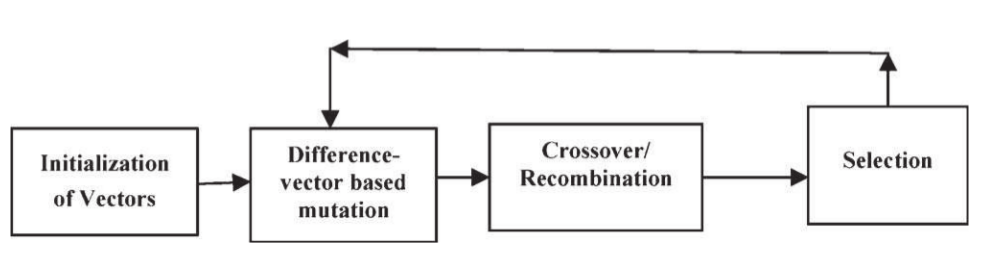
\includegraphics[scale=0.3]{Figures/DEop.png}
	\caption{The optimization process of DE \cite{das2011differential}.}\label{img:DE}
\end{figure}

The optimization process of DE the works through a simple cycle of stages, presented in Figure \ref{img:DE}, that we can summarize as follows:

\begin{itemize}
	
	\item \textbf{Initialization of Vectors}: DE begins with a randomly initialized population of a given number of $D$-dimensional arrays of parameters. These vectors constitute candidate solutions for the problem to be solved.
	
	\item \textbf{Difference-vector-based mutation}: DE introduces diversity into the population via the mutation operator. This operator is applied to each individual of the population, known in this context as the parent vector. It combines the parent vector with two randomly selected vectors from the population by applying an arithmetic operator to them. The result of this process is a mutant vector.
	
	\item \textbf{Crossover/Recombination}: The mutant vector exchanges some components with its associated parent to form a trial vector, which will be the candidate to replace the parent vector. Several strategies exist to generate this trial vector, which we will not delve into; however, they can be found in \cite{das2011differential}.
	
	\item \textbf{Selection}: The newly generated trial vector is compared with its associated parent using the fitness function. If the trial vector is better than the parent, then it will replace the parent in the next generation. It is worth noting that, following this strategy, the population never degenerates but only gets better or remains the same.
	
\end{itemize}

Even though DE was a major breakthrough in terms of real optimization, many variants have been developed since its invention that provide better results. We will focus on the SHADE variant, which adaptively optimizes some of the parameters of DE (see Section \ref{sec:SHADE}).

\section{Brief Review of the BRKGA Algorithm} \label{sec:brkga}

The biased random-key genetic algorithm---from now on BRKGA---was first proposed in \cite{gonccalves2011biased} as a generalization of the random-key genetic algorithm \cite{bean1994genetic}.

In BRKGA, each solution---also called individual---is represented as a vector of values within the interval $[0,1]$. However, this vector is not a solution to the problem but a representation of it. This allows us to abstract the details of the problem in order to apply a genetic algorithm that operates with real coding. Therefore, a deterministic decoder is necessary to obtain the actual solution to the problem from the vector that encodes it.

BRKGA also requires a fitness function to evaluate each individual. This function takes the decoded solution as input and provides its fitness value as output. It is designed specifically for each problem.

The BRKGA optimization process is completely independent of the problem to solve. First, a population $P$ of $p_{size}$ vectors of random-keys is initialized, and this will be the initial generation. Each random-key vector $p_i$ has $N$ random-keys in it. The population is sorted by the fitness value $f_i$ of each $p_i$ to select the first $p_e$ individuals, this is, the elite of the population. The elite will be preserved in the next generation without modification. To introduce diversity, a number $p_m$ of new random-keys vectors are also included in the next generation. The remaining individuals of the new generation ($p_{size} - p_e - p_m$) are obtained through crossovers between elite and non-elite parents \cite{de2017comparison}.

\subsection{Adaptation of BRKGA for Constrained Clustering} \label{sec:AdaptationofBRKGA}

An adaptation of BRKGA for constrained clustering was proposed in \cite{de2017comparison}.

This method randomly initializes a population of random-key vectors, each one with $n$ random-keys. The decoder divides the interval $[0,1]$ in $k$ intervals, so there exists a correspondence between each random-key (instance $x_i$) and the integer (label $l_i$) corresponding to the interval which it lies in. Table \ref{tab:decodingrk} shows an example of random-key decoding for a dataset with 10 instances ($n$ = 10) and $k = 3$. Note that extreme values 0 and 1 can also appear in a random-key vector.

\begin{table}[!h]
	\centering
	%\setlength{\arrayrulewidth}{1mm}
	\setlength{\tabcolsep}{7pt}
	\renewcommand{\arraystretch}{1.2}
	\resizebox{\textwidth}{!}{
	\begin{tabular}{|c|c|c|c|c|c|c|c|c|c|c|}
		\hline
		Index (instance) & 1 & 2 & 3 & 4 & 5 & 6 & 7 & 8 & 9 & 10 \\
		\hline
		Random-key & 0.12 & 0.37 & 0.66 & 0.56 & 0.00 & 0.97 & 0.23 & 0.25 & 0.15 & 1.00 \\
		\hline
		Cluster (label) & 1 & 2 & 2 & 2 & 1 & 3 & 1 & 3 & 1 & 3 \\
		\hline

	\end{tabular}}
	\caption{Random-key decodification example \cite{de2017comparison}}
	\label{tab:decodingrk}
\end{table}

Once the decoded solution has been obtained, the fitness value of the solution is computed as in Equation \eqref{eq1}.

\begin{equation}
f_i = z_i + \overbrace{(\mu * n * {infeasibility}_i)}^{penalty},
\label{eq1}
\end{equation}

\noindent where $\mu$ is a high value, $infeasibility_i$ is the number of non-satisfied constraints and $z_i$ is the within-cluster-sum-of-squares which can be computed as in Equation \eqref{eq2}.

\begin{equation}
z_i = \sum_{c_j \in C_i} \left[ \frac{\sum_{x_a, x_b \in c_j} d^2(x_a,x_b)}{|c_j|}\right],
\label{eq2}
\end{equation}

\noindent where $C_i$ is the partition of dataset $X$ defined by solution (individual) $p_i$, and $(x_a, x_b)$ are instances in the cluster $c_j$ such that $a \neq b$ and the Euclidean distance ($d^2(\cdot, \cdot)$) between each pair of instances in $C_i$ is included in the sum only once.

In \cite{de2017comparison}, the authors also added a new element to BRKGA, a local search procedure. This local optimization method is applied to each decoded individual in each generation, but its results are not transferred to the individual, so that diversity is maintained. Thus, the individuals produced by the local search are only used to update the best solution found so far if needed. For more details on BRKGA see \cite{de2017comparison}.

\section{The SHADE Optimization Method} \label{sec:SHADE}

Success History Based Adaptive Differential Evolution (SHADE) is an optimization method based on differential evolution. Proposed in \cite{tanabe2013success}, it was an improvement for the JADE model, presented in \cite{zhang2009jade}.

Unlike JADE, which only considers the parameters used in the previous generation, SHADE uses a historical record of successful parameters as a mechanism for adapting parameters involved in the process of creating new generations.

\subsection{SHADE Operators}

As in differential evolution, SHADE employs mutant generation, crossover and replacement operators to explore the space of solutions and bring in new generations of individuals.

The mutation strategy used by SHADE is known as current-to-$p$best/1, and the expression that generates new individuals is described in Equation \eqref{eq3}.

\begin{equation}
m_{[i,G]} = p_{[i,G]} + F_i * (p_{[pbest, G]} - p_{[i,G]}) + F_i * (p_{[r1, G]} - p_{[r2,G]}),
\label{eq3}
\end{equation}

\noindent where $m_{[i,G]}$ is the mutant vector, which is generated with an individual $p_{[i,G]}$ from the population serving as a starting point. Indices $r1$ and $r2$ are random values in the range $[0,p_{size}]$, different from $i$ and from each other. The individual $p_{[pbest, G]}$ is randomly selected from among the best $N \times pbest\;|\;pbest\in [0,1]$ individuals in the population. This way, the parameter $pbest$ controls the greediness of the mutation strategy. The parameter $F_i$ defines the magnitude of the operator.

After generating the mutant vector $m_{[i,G]}$, it is combined with the parent $p_{[i,G]}$ vector by means of a crossover operator; the result is the trial vector. SHADE uses the Binomial crossover operator, which is defined by the Equation \eqref{eq4}.

\begin{equation}
t_{[j,i,G]} = \left\{ \begin{array}{lc}
m_{[j,i,G]} &   if \;\; \text{rand}[0,1) \le CR_i \;\; or \;\;j = j_{rand} \\
p_{[j,i,G]} &  \text{otherwise}
\end{array}
\right.,
\label{eq4}
\end{equation}

\noindent where $rand[0,1)$ is a random number selected from a normal distribution in the range $[0,1)$, $j_{rand}$ is a random integer selected from the range $[1,D]$, and $CR \in [0,1]$ is the crossover ratio.

The SHADE replacement operator determines the survivors individuals for the next generation. It compares each parent $x_{[i,G]}$ with the trial vector $_{[j,i,G]}$, generated based on it. The best one of these two individuals will survive for the next generation. Equation \eqref{eq5} shows this concept.

\begin{equation}
p_{[i,G + 1]} = \left\{ \begin{array}{lc}
t_{[i,G]} &   if \;\; f(t_{[i,G]}) \le f(p_{[i,G]}) \\
p_{[i,G]} &  \text{otherwise}
\end{array}
\right.
\label{eq5}
\end{equation}

To maintain diversity, SHADE can make use of an external archive $A$, in which parents $p_{[i,G]}$ who were replaced by their associated trial vector $t_{[i,G]}$ are saved. To make use of the archive, we will consider that the individual $p_{[r2,G]}$ from Equation \eqref{eq3} is selected from $P \cup A$. The archive size is the same as the population size. When the size of $A$ exceeds the size of $P$, random individuals are selected for removal to make room for new ones.

The parameters $pbest$, $F_i$ and $CR_i$ are difficult to adjust and their selection is not trivial, as they largely determine the success of the optimization process. These are the parameters that SHADE adaptively optimizes using the mentioned history record.

\subsection{SHADE Parameter Adaptation Method}

The SHADE method stores in memory a structure with $H$ entries for parameters $F_i$ and $CR_i$, as shown in Table \ref{tab:SHADEmemory}. This structure is initialized with the value $0.5$ for all entries.

\begin{table}[!h]
	\centering
	%\setlength{\arrayrulewidth}{1mm}
	\setlength{\tabcolsep}{13pt}
	%\renewcommand{\arraystretch}{0.9}
	\resizebox{\textwidth}{!}{
	\begin{tabular}{|c|c|c|c|c|c|}
		\hline
		 Index & 1 & 2 & $\cdots$ & $H - 1$ & $H$ \\
		 \hline
		 \hline
		 $M_{CR}$ & $M_{[CR,1]}$ & $M_{[CR,1]}$ & $\cdots$ & $M_{[CR,H-1]}$ & $M_{[CR,H]}$ \\
		 \hline
		 $M_{F}$ & $M_{[F,1]}$ & $M_{[F,1]}$ & $\cdots$ & $M_{[F,H-1]}$ & $M_{[F,H]}$ \\
		\hline

	\end{tabular}}
	\caption{Historical memory $M_{CR}$, $M_{F}$ used by SHADE \cite{tanabe2013success}}
	\label{tab:SHADEmemory}
\end{table}

In each generation, parameters $CR_i$ and $F_i$ are calculated on the basis of the existing history by applying Equations \eqref{eq6} and \eqref{eq7}:

\begin{equation}
CR_i = \text{randn}_i(M_{[CR,r_i]}, 0.1)
\label{eq6}
\end{equation}

\begin{equation}
F_i = \text{randc}_i(M_{[F,r_i]}, 0.1),
\label{eq7}
\end{equation}

\noindent where $randn(\mu, \sigma^2)$ and $randc(\mu, \sigma^2)$ are random values from normal and Cauchy distributions respectively, with mean $\mu$ and variance $\sigma^2$. When a value for $CR_i$ outside of the range $[0,1]$ is generated, it is replaced by the corresponding limit value. If $F_i > 1$, then it is truncated to $1$; conversely, if $F_i < 0$, then Equation \eqref{eq7} is applied as many times as needed to obtain a legal value.

SHADE keeps two auxiliary sets $S_{CR}$ and $S_F$ to store the $CR_i$ and $F_i$ values that were successfully used to generate a trial vector that replaced the parent. At the end of each generation, the content of the memory $M$ is updated following Equations \eqref{eq8} and \eqref{eq9}.

\begin{equation}
M_{[CR,h,G+1]} = \left\{ \begin{array}{lc}
\text{mean}_{WA} (S_{CR}) &   if \;\; S_{CR} \neq \emptyset \\
M_{[CR,h,G+1]} &  otherwise
\end{array}
\right.
\label{eq8}
\end{equation}

\begin{equation}
M_{[F,h,G+1]} = \left\{ \begin{array}{lc}
\text{mean}_{WL} (S_{F}) &   if \;\; S_{F} \neq \emptyset \\
M_{[F,h,G+1]} &  otherwise
\end{array}
\right.
\label{eq9}
\end{equation}

The $h \;\; (0 \le h \le H)$ index specifies the position of the memory $M$ to be updated. This index is initialized to $0$ at the beginning of the optimization process and increased by one after every generation. When $h \ge H$ then $h$ is reset to 1. It is worth noting that, when there is a generation with no trial vectors successfully replacing their parents, no update of $M$ is done.

In Equation \ref{eq8}, the term $mean_{WA} (S_{CR})$ is the weighted mean, which is computed following Equations \eqref{eq10} and \eqref{eq11}, proposed in \cite{peng2009multi} to prevent $CR$ from converging to small values.

\begin{equation}
\text{mean}_{WA} (S_{CR}) = \sum_{i = 1}^{|S_{RC}|} \omega_i * S_{[RC,i]}
\label{eq10}
\end{equation}

\begin{equation}
\omega_i = \frac{\Delta f_i}{\sum_{i = 1}^{|S_{RC}|} \Delta f_i},
\label{eq11}
\end{equation}

\noindent where $\Delta f_i = |f(t_{[i,G]}) - f(p_{[i, G]})|$, which is the amount of improvement obtained from the trial vector with respect to the parent.

In Equation \ref{eq9} the term $mean_{WL} (S_{F})$ refers to the weighted Lehmer mean, which is computed as in Equation \eqref{eq12} (proposed in \cite{tanabe2013success}).

\begin{equation}
\text{mean}_{WL} (S_{F}) = \frac{\sum_{i = 1}^{|S_{F}|} \omega_i * S^2_{[F,i]}}{\sum_{i = 1}^{|S_{F}|} \omega_i * S_{[F,i]}}
\label{eq12}
\end{equation}

Unlike parameters $S_{CR}$ and $S_F$, the parameter $pbest$ from Equation \eqref{eq3}, used to set the greediness of the mutation strategy, is not included in the adaptive optimization process. However, it is not static: it is calculated for every individual $p_i$ of the population following Equation \eqref{eq13}.

\begin{equation}
pbest_i = \text{randn}[2/N, 0.2],
\label{eq13}
\end{equation}

\noindent such that there is always at least two individuals to choose between.

\subsection{Adaptation of SHADE for constrained clustering} \label{sec:SHADEadapt}

For the adaptation of SHADE to the problem of constrained clustering, we will take some of the elements that allowed us to adapt it to BRKGA. To begin with, we will use random-keys to create the individuals of the population; this way, each individual is defined as a vector of $n$ random-keys. Additionally, we will also reuse the same initialization method and the same decoder used in BRKGA (see Section \ref{sec:AdaptationofBRKGA}).

However, we propose a new fitness function to evaluate the quality of the individuals of the population, Equation \eqref{eq14}, whose element $z_i$ is obtained as in Equation \eqref{eq2}.

\begin{equation}
f_i = z_i * (infeasibility + 1)
\label{eq14}
\end{equation}

Note that in Equation \eqref{eq14} no parameter is involved that cannot be calculated from the dataset or constraints, whereas in Equation \eqref{eq1} the $\mu$ parameter must be calculated and optimized for each individual problem.

We found that with the fitness function defined in \eqref{eq1} there is no competition between the penalty term and the within-cluster-sum-of-squares term, because the penalty is always significantly larger than it or zero. This can bias the exploration of the solution space, restricting it in practice to those that satisfy all the constraints, even if the within-cluster-sum-of-squares is still improvable by moving two instances involved in a constraint to different clusters without violating that constraint.

With Equation \eqref{eq14} we try to find a trade-off between the within-cluster-sum-of-squares and the penalty term, allowing solutions that violate a certain number of constraints to compete with those who violate a smaller number of them but score a better within-cluster-sum-of-squares.

To make these concepts clear we consider a toy dataset and three partitions over it. The dataset from Figure \ref{img:toydatasets} contains 100 instances and a single ML constraint between two instances from the same class. Partitions $C_0$---displaying the true labels---and $C_1$ do not violate the constraint ($infeasibility = 0$), whereas $C_2$ does violate it ($infeasibility = 1$). However, $C_2$ shows a possibility, for later iterations, of adding both instances to their nearest cluster while also satisfying the ML constraint.

\begin{figure}[bth]
	\myfloatalign
	{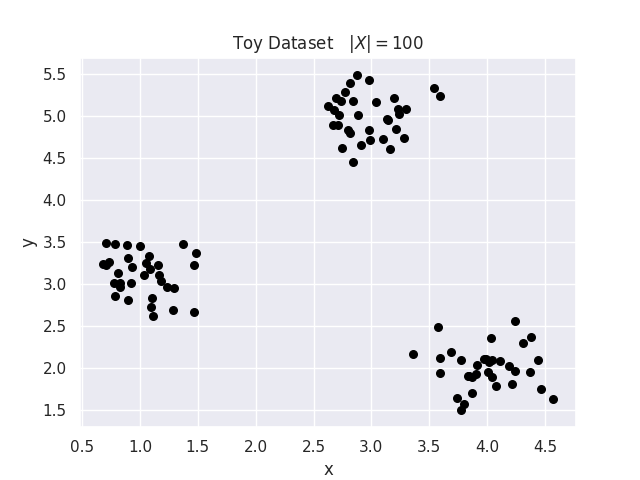
\includegraphics[width=.45\linewidth]{Figures/Dataset}} \quad
	%\subfloat[Imagen original]
	{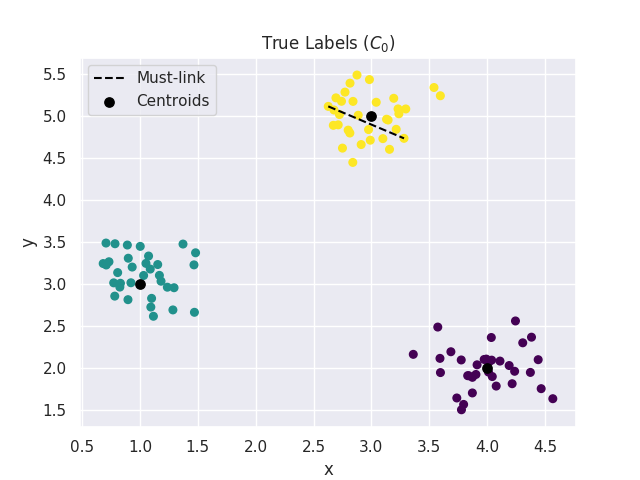
\includegraphics[width=.45\linewidth]{Figures/C0}} \quad
	%\subfloat[Clustering sin restricciones]
	{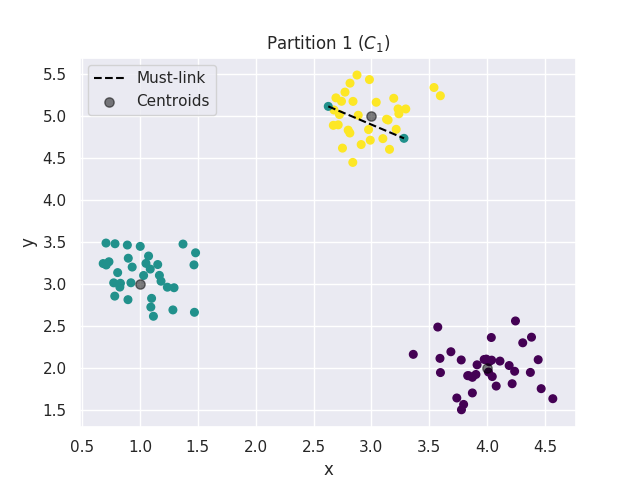
\includegraphics[width=.45\linewidth]{Figures/C1}} \quad
	%\subfloat[Clustering con restricciones]
	{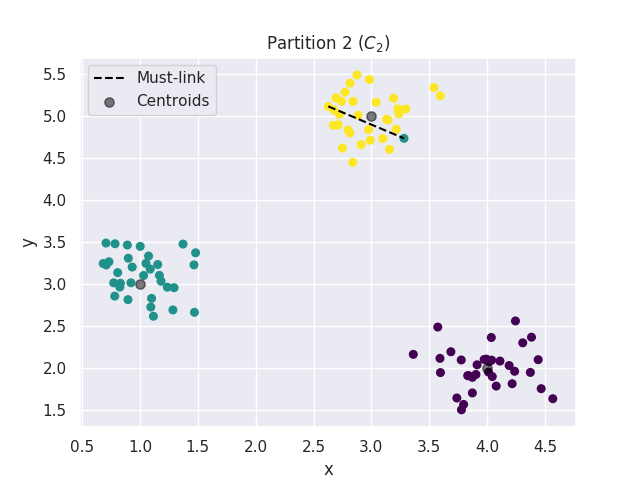
\includegraphics[width=.45\linewidth]{Figures/C2}} \quad
	\caption{Three partitions over a toy dataset.}
	\label{img:toydatasets}
\end{figure}

Table \ref{tab:fitnessfunctions} shows fitness values for each partition from Figure \ref{img:toydatasets}. We refer to the function presented in Equation \eqref{eq1} as $f_1$ and to the function presented in Equation \eqref{eq14} as $f_2$.

\begin{table}[!h]
	\centering
	\setlength{\tabcolsep}{7pt}
	\renewcommand{\arraystretch}{1.3}
	%\begin{adjustwidth}{-1in}{-1in}
	\resizebox{\textwidth}{!}{
		\begin{tabular}{c c c c c c}
			\hline
			\multirow{2}{*}{Partition} &
			\multicolumn{2}{c}{Expression} &&
			\multicolumn{2}{c}{Value} \\
			\cline{2-3} \cline{5-6}
			& $f_1$ & $f_2$ && $f_1$ & $f_2$ \\
			\hline
			$C_0$ & $z_0$ & $z_0$ && $0.457$  & $0.457$  \\
			$C_1$ & $z_1$ & $z_1$ && $0.540$  & $0.540$  \\
			$C_2$ & $z_2 + (\mu * N * infs)$ & $z_2 * (infs + 1)$  && $0.503 + 1000 = 1000.503$ &  $0.503 * 2 = 1.005$ \\
			\hline

		\end{tabular}}
		%\end{adjustwidth}

	\caption{Expression and value of fitness functions over three partitions. ($\mu = 10$)}
	\label{tab:fitnessfunctions}
\end{table}

Results in Table \ref{tab:fitnessfunctions} are a clear example of the above. In the general case, by using $f_2$ the penalty for violating constraints is proportional to the within-cluster-sum-of-squares---the lower it is, the lower the penalty. This is not the case with $f_1$, whose penalty term is independent of the within-cluster-sum-of-squares, which can result in a difference of several orders of magnitude between partitions satisfying different amounts of constraints.

As in \cite{de2017comparison} we apply a local optimization procedure to the individuals of the population, but without transferring its results to the original individual in order to maintain diversity. The difference is that we do not apply it to the whole population but only to a number $p_e$ of individuals considered as the elite of the population. The percentage of individuals considered as elite must be determined for each case.

Algorithm \ref{alg:SHADE} describes the overall SHADE optimization process and it is an adaptation of the one that can be found in \cite{tanabe2013success} to include the local search procedure presented in Algorithm \ref{alg:LS}.

\begin{algorithm}
	\SetNlSty{textbf}{[}{]}
	\SetNlSkip{0.5em}
	\setstretch{1.2}
	\SetKwFunction{Sort}{Sort}
	\SetKwFunction{LocalSearch}{LocalSearch}
	\KwIn{Dataset $X$, constraint sets $C_=$ and $C_{\neq}$, population size $p_{size}$, elite size $p_e$, number of clusters $K$.}
	\tcp{Initialization phase}
	$G \leftarrow 0$\\
	Initialize population $P_0 \leftarrow \{p_{[1,0]}, \cdots, p_{[p_{size},0]}\}$\\
	Initialize all values in $M_{CR}$, $M_F$ to 0.5\\
	$A \leftarrow \emptyset$; $h \leftarrow 1$\\
	\tcp{Main loop}
	\While{Termination criteria are not met}{

		$S_{CR} \leftarrow S_F \leftarrow \emptyset$\\
		$P_G \leftarrow$ \Sort{$P_G$} \tcp{Sort the population}
		\tcp{Apply a LS procedure to the elite of the population}
		\LocalSearch{$\{p_{[1,G]}, \cdots, p_{[p_{e},G]}\}$}\\
		\For{$i \in [1,p_{size}]$}{
			$r_i \leftarrow$ randInt$[1,H]$\\
			$CR_{[i,G]} \leftarrow$ randn$_i(M_{[CR,r_i]}, 0.1)$\\
			$F_{[i,G]} \leftarrow$ randc$_i(M_{[F,r_i]}, 0.1)$\\
			$p_{[i,G]} \leftarrow$ rand$[N/2, 0.2]$\\
			Generate trial vector $t_{[i,G]}$ by current-to-$p$best/1/bin\\

			\eIf{$f(t_{[i,G]}) \le f(p_{[i,G]})$}{
				$p_{[i,G + 1]} \leftarrow t_{[i,G]}$
			}{
				$p_{[i,G + 1]} \leftarrow p_{[i,G]}$
			}

			\If{$f(t_{[i,G]}) < f(p_{[i,G]})$}{
				$p_{[i,G]} \rightarrow A$;
				$CR_{[i,G]} \rightarrow S_{CR}$;
				$F_{[i,G]} \rightarrow S_{F}$
			}

		}
		Whenever $|A| > |P|$, randomly select an individual from $A$ to be deleted so that $|A| \le |P|$\\
		\If{$S_{CR} \neq \emptyset$ \textbf{and} $S_{F} \neq \emptyset$}{
			Update $M_{[CR,h]}$ and $M_{[F,h]}$ based on $S_{CR}$ and $S_{F}$\\
			$h \leftarrow (h + 1) \mod H$
		}
		$G++$
	}
	\caption{Modified SHADE}\label{alg:SHADE}
\end{algorithm}

\begin{algorithm}
	\SetNlSty{textbf}{[}{]}
	\SetNlSkip{0.5em}
	\setstretch{1.2}
	\SetKwFunction{RandomShuffle}{RandomShuffle}
	\SetKwRepeat{Do}{do}{while}
	\KwIn{Dataset $X$, constraint sets $C_=$ and $C_{\neq}$, decoded random-key vector (solution) $S$, number of clusters $K$.}
	\BlankLine
	\While{$improvement$}{
		$improvement \leftarrow$ \texttt{false} \\

		$s_i \leftarrow $ Select random object from $S$\\
		\tcp{Random shuffle labels set}
		$RSL \leftarrow $ \RandomShuffle{$\{1,\cdots,K\}$}\\
		\For{$c \in RSL$}{
			$S^\prime \leftarrow S$\\
			$S^\prime$\texttt{[}$s_i$\texttt{]} $\leftarrow c$ \tcp{Move object $s_i$ to cluster $c$}

			\If{$f(S^\prime) < f(S)$}{
				$S \leftarrow S^\prime$\\
				$improvement \leftarrow$ \texttt{true} \\
			}
		}
	}
	\BlankLine
	\KwRet ($S$)

\caption{Local Search}\label{alg:LS}
\end{algorithm}

\clearpage

\section{Experimental Setup} \label{sec:expSetup}

For our experiments we will compare the results obtained by BRKGA and SHADE over 25 datasets. Most of these datasets can be found at the \href{https://sci2s.ugr.es/keel/category.php?cat=clas}{Keel-dataset repository}\cite{triguero2017keel}, though some of them have been obtained via
\href{https://scikit-learn.org/stable/datasets/index.html}{\texttt{scikit-learn} python package} \cite{scikit-learn}. We also include 3 artificial datasets in our analysis, namely: \textit{Circles}, \textit{Moons} and \textit{Spiral}, which can be found at GitHub. Table \ref{tab:datasets} displays a summary of every dataset.

\begin{table}[!h]
	\centering
	%\setlength{\arrayrulewidth}{1mm}
	%\setlength{\tabcolsep}{5pt}
	%\renewcommand{\arraystretch}{1.2}
	%\resizebox{\textwidth}{!}{
	\small
	\begin{tabular}{l c c c}
		\hline
		Name & No. Instances & No. Classes & No. Features \\
		\hline
		Appendicitis & 106 & 2 & 7 \\
		Boston & 506 & 229 & 13 \\
		Breast Cancer & 569 & 2 & 30 \\
		Circles & 300 & 2 & 2 \\
		Diabetes & 442 & 214 & 10 \\
		Ecoli & 336 & 8 & 7 \\
		Glass & 214 & 6 & 9 \\
		Haberman & 306 & 2 & 3 \\
		Hayesroth & 160 & 3 & 4 \\
		Ionosphere & 351 & 2 & 33 \\
		Iris & 150 & 3 & 4 \\
		Led7Digit & 500 & 10 & 7 \\
		Monk2 & 432 & 2 & 6 \\
		Moons & 300 & 2 & 2 \\
		Pima & 768 & 2 & 8 \\
		Saheart & 462 & 2 & 9 \\
		Sonar & 208 & 2 & 60 \\
		Soybean & 47 & 4 & 35 \\
		Spectfheart & 267 & 2 & 44 \\
		Spiral & 300 & 2 & 2 \\
		Tae & 151 & 3 & 5 \\
		Vehicle & 846 & 4 & 18 \\
		Vowel & 990 & 11 & 13 \\
		Wdbc & 569 & 2 & 30 \\
		Zoo & 101 & 7 & 16 \\
		\hline

	\end{tabular}%}
	\caption{Summary of datasets used for the experiments \cite{triguero2017keel}\cite{scikit-learn}}
	\label{tab:datasets}
\end{table}

\clearpage

\subsection{Constraint Generation}

Since we have the true labels associated with each dataset, we will use the method proposed in \cite{wagstaff2001constrained} to generate artificial constraint sets. This method consists in randomly selecting two instances of a dataset, then comparing its labels, and finally setting an ML or CL constraint depending on whether the labels are the same or different.

We will generate, for each dataset, three different sets of constraints---$CS_{10}$, $CS_{15}$ and $CS_{20}$---that will be associated with four small percentages of the size of the dataset: 10\%, 15\% and 20\%. With $n$ being the fraction of the size of the dataset associated to each of these percentages, the formula $\frac{n(n-1)}{2}$ tells us how many artificial constraints will be created for each constraint set; this number is equivalent to how many edges a complete graph with $n$ vertices would have.

The random allocation of constraints has a potential advantage over simply using the constraints contained in an $n$-vertex complete graph: there is a lower probability of biasing the constraint set towards having classes with poor representation in it. Table \ref{tab:constraints} shows the number of constraints of each type obtained for each dataset.

\begin{table}[!h]
	\centering
	\setlength{\tabcolsep}{7pt}
	\renewcommand{\arraystretch}{1.2}
	%\begin{adjustwidth}{-1in}{-1in}
	\resizebox{\textwidth}{!}{
	\begin{tabular}{lcc c cc c cc}
		\hline
		\multirow{2}{*}{Dataset} &
		\multicolumn{2}{c}{$CS_{10}$} && \multicolumn{2}{c}{$CS_{15}$} && \multicolumn{2}{c}{$CS_{20}$} \\
		\cline{2-3} \cline{5-6} \cline{8-9}
		& ML & CL && ML & CL && ML & CL \\
		\hline
		Appendicitis & 39 & 16 && 71 & 49 && 164 & 67 \\
		Boston & 3 & 1272 && 13 & 2837 && 26 & 5125 \\
		Breast Cancer & 876 & 720 && 1965 & 1690 && 3487 & 2954 \\
		Circles & 208 & 227 && 502 & 488 && 853 & 917 \\
		Diabetes & 5 & 985 && 7 & 2204 && 23 & 3893 \\
		Ecoli & 163 & 398 && 357 & 918 && 609 & 1669 \\
		Glass & 52 & 179 && 139 & 389 && 259 & 644 \\
		Haberman & 304 & 161 && 634 & 401 && 1135 & 756 \\
		Hayesroth & 39 & 81 && 102 & 174 && 177 & 319 \\
		Ionosphere & 330 & 300 && 732 & 646 && 1299 & 1186 \\
		Iris & 26 & 79 && 82 & 171 && 136 & 299 \\
		Led7Digit & 126 & 1099 && 267 & 2508 && 460 & 4490 \\
		Monk2 & 473 & 473 && 979 & 1101 && 1917 & 1824 \\
		Moons & 200 & 235 && 494 & 496 && 900 & 870 \\
		Pima & 1604 & 1322 && 3595 & 3075 && 6452 & 5329 \\
		Saheart & 595 & 486 && 1292 & 1123 && 2330 & 1948 \\
		Sonar & 100 & 110 && 245 & 251 && 436 & 425 \\
		Soybean & 4 & 6 && 6 & 22 && 12 & 33 \\
		Spectfheart & 233 & 118 && 543 & 277 && 965 & 466 \\
		Spiral & 224 & 211 && 487 & 503 && 918 & 852 \\
		Tae & 40 & 80 && 82 & 171 && 151 & 314 \\
		Vehicle & 874 & 2696 && 1955 & 6046 && 3589 & 10776 \\
		Vowel & 445 & 4406 && 1026 & 10000 && 1705 & 17798 \\
		Wdbc & 840 & 756 && 1925 & 1730 && 3472 & 2969 \\
		Zoo & 21 & 34 && 29 & 91 && 41 & 169 \\
		\hline

	\end{tabular}}
	%\end{adjustwidth}

	\caption{Number of constraints used in experiments}
	\label{tab:constraints}
\end{table}

Note that the greater the number of classes present in the dataset, the fewer ML constraints obtained with the method proposed in \cite{wagstaff2001constrained}. This is because the probability of randomly choosing two individuals from the same class decreases as the number of classes present in the dataset increases.

\clearpage

\subsection{Evaluation Method}

Since we have the true labels associated to each of the datasets, we can use them in post-processing to evaluate the results provided by each method. We will use the Adjusted Rand Index to measure the accuracy of the predictions resulting from each method we test \cite{hubert1985comparing}. The Basic Rand Index computes the degree of agreement between two partitions $C_1$ and $C_2$ of a given dataset $X$. $C_1$ and $C_2$ are viewed as collections of $N(N - 1)/2$ pairwise decisions \cite{rand1971objective}.

For each pair of instances $x_i$ and $x_j$ in $X$, $C_i$ assigns them to the same cluster or to different clusters. We take $a$ as the number of pairings where $x_i$ is in the same cluster as $x_j$ in both $C_1$ and $C_2$, and $b$ as the opposite event ($x_i$ and $x_j$ are in different clusters in $C_1$ and $C_2$). Then, the degree of similarity between $C_1$ and $C_2$ is calculated as in Equation \eqref{eq15}.

\begin{equation}
Rand(C_1, C_2) = \frac{a + b}{N(N - 1)/2}
\label{eq15}
\end{equation}

The Adjusted Rand Index is a corrected-for-chance version of the Rand Index. This correction uses the expected similarity of all comparisons between clusterings specified by a random model to set up a baseline. The Adjusted Rand Index is computed as in Equation \eqref{eq16}.

\begin{equation}
ARI(C_1, C_2) = \frac{Rand(C_1, C_2) - ExpectedIndex}{MaximumIndex - ExpectedIndex},
\label{eq16}
\end{equation}

\noindent where $MaximumIndex$ is expected to be 1 and $ExpectedIndex$ is the already mentioned expected degree of similarity with a random model. It is easy to see that $ARI(C_1, C_2) \in [-1,1]$, such that an $ARI$ value close to 1 means a high degree of agreement between $C_1$ and $C_2$, a positive value close to 0 means no agreement and a value smaller that 0 means that the $Rand(C_1, C_2)$ is less than expected when comparing with random partitions. To summarize, the higher the $ARI$, the greater the degree of similarity between $C_1$ and $C_2$. For more details on Adjusted Rand Index see \cite{hubert1985comparing}.

%% CORREGIR DESDE AQUI HASTA EL FINAL

\subsection{Calibration}

Table \ref{tab:params} shows a summary of the parameter setup used for both BRKGA+LS and SHADE+LS algorithms.

\begin{table}[!h]
	\centering
	\setlength{\tabcolsep}{7pt}
	\renewcommand{\arraystretch}{1.4}
	%\begin{adjustwidth}{-1in}{-1in}
	\resizebox{\textwidth}{!}{
		\begin{tabular}{>{\centering\arraybackslash}c m{5cm} cc}
			\hline
			Parameter & Meaning & BRKGA & SHADE \\
			\hline
			$p_{size}$ & Population size & 100 & 100 \\
			$Evals$ & Fitness function evaluations & 300000 & 300000 \\
			$p_e$ & Size of the elite set in population & $0.2 * p_{size}$ & $0.25 * p_{size}$ \\
			$p_m$ & Number of mutants to be introduced in the population in each generation & $0.2 * p_{size}$ & - \\
			$p_{inherit}$ & Probability that a feature is inherited from an elite parent & $50\%$ & - \\
			$K$ & Output partition number of clusters & \multicolumn{2}{m{4cm}}{Known for each dataset (Table \ref{tab:datasets}). It has the same value for both methods} \\
			\hline

		\end{tabular}}
		%\end{adjustwidth}

		\caption{Parameters setup used for BRKGA and SHADE.}
		\label{tab:params}
	\end{table}
	
In both cases---BRKGA+LS and SHADE+LS---the population size will be 100 individuals, and the stop criterion is given by the number of evaluations of the fitness function, which at most will be 300000.
	
To compare with the state-of-the-art methods mentioned in section \ref{sec:BackSOTA} we will use the parameters recommended by the authors, setting the maximum limit of iterations as 300 in all cases.

It should be noted that the study presented in this document aims to compare average performance, not peak performance. The parameter optimization process required for each algorithm and dataset falls outside the scope of this study.

\section{Experimental Results} \label{sec:results}

In this section we present Tables \ref{tab:results10} to \ref{tab:results20SOTA}, which display the results obtained by the methods to be compared for each dataset and constraint set.

Since the methods we are comparing involve non-deterministic procedures, the results may vary from one run to another. To lessen the effect this may have on the results, we will apply each method 5 times to every dataset and constraint set, so that the measures shown in the previously mentioned tables correspond to the average of the 5 runs.

\subsection{Comparing BRKGA+LS with SHADE+LS}

In Tables \ref{tab:results10} to \ref{tab:results20} the ARI columns shows the Adjusted Rand Index for each case, the Unsat columns displays the percentage of violated constraints and the Time columns shows the time taken for each algorithm to deliver results, measured in seconds.

\begin{table}[!h]
	\centering
	\setlength{\tabcolsep}{7pt}
	\renewcommand{\arraystretch}{1.4}
	%\begin{adjustwidth}{-1in}{-1in}
	\resizebox{\textwidth}{!}{
		\begin{tabular}{l ccc c ccc}
			\hline
			\multirow{2}{*}{Dataset} &
			\multicolumn{3}{c}{BRKGA+LS} &&  \multicolumn{3}{c}{SHADE+LS} \\
			\cline{2-4} \cline{6-8}
			& ARI & Unsat(\%) & Time(s) && ARI & Unsat(\%) & Time(s) \\
			\hline
			Appendicitis & 0.022 & 5.454 & 383.642 && 0.086 & 5.091 & 366.491 \\
			Boston & -0.000 & 0.173 & 1502.452 && -0.001 & 0.235 & 1570.547 \\
			Breast\_Cancer & 0.395 & 17.444 & 3651.263 && 0.159 & 22.256 & 3602.665 \\
			Circles & 0.166 & 12.598 & 1077.238 && 0.063 & 14.207 & 1060.787 \\
			Diabetes & 0.000 & 0.364 & 1277.982 && 0.003 & 0.465 & 1284.486 \\
			Ecoli & 0.009 & 20.321 & 1169.798 && 0.020 & 12.763 & 1112.981 \\
			Glass & 0.016 & 8.658 & 735.507 && 0.013 & 4.848 & 694.962 \\
			Haberman & 0.047 & 15.699 & 1155.985 && 0.084 & 15.441 & 1146.023 \\
			Hayesroth & 0.027 & 1.500 & 550.117 && 0.025 & 2.000 & 529.424 \\
			Ionosphere & 0.125 & 17.587 & 1894.390 && 0.332 & 12.603 & 1872.308 \\
			Iris & 0.238 & 0.190 & 505.112 && 0.342 & 0.000 & 483.584 \\
			Led7Digit & 0.009 & 11.347 & 1786.943 && 0.004 & 8.866 & 1784.708 \\
			Monk2 & 0.421 & 14.926 & 1848.543 && 0.270 & 16.385 & 1821.208 \\
			Moons & 0.277 & 11.816 & 1098.089 && 0.272 & 11.356 & 1075.089 \\
			Pima & 0.236 & 25.195 & 4072.087 && 0.275 & 22.468 & 3990.383 \\
			Saheart & 0.147 & 20.555 & 2135.624 && 0.265 & 16.725 & 2095.554 \\
			Sonar & 0.124 & 7.619 & 1106.039 && 0.116 & 8.952 & 1081.994 \\
			Soybean & 0.496 & 0.000 & 176.333 && 0.515 & 0.000 & 151.163 \\
			Spectfheart & 0.334 & 9.573 & 1451.235 && 0.343 & 8.604 & 1405.243 \\
			Spiral & 0.058 & 15.402 & 1098.622 && 0.114 & 13.793 & 1099.747 \\
			Tae & 0.018 & 0.833 & 520.855 && 0.024 & 1.333 & 508.988 \\
			Vehicle & 0.005 & 28.515 & 4366.104 && 0.006 & 22.151 & 4352.663 \\
			Vowel & 0.003 & 13.330 & 4245.672 && 0.002 & 11.523 & 4290.154 \\
			Wdbc & 0.478 & 16.316 & 3596.517 && 0.357 & 17.093 & 3528.029 \\
			Zoo & 0.105 & 1.091 & 336.345 && 0.098 & 2.182 & 317.674 \\
			\hline

		\end{tabular}}
		%\end{adjustwidth}

	\caption{Experimental results obtained for $CS_{10}$ comparing SHADE+LS and BRKGA+LS}
	\label{tab:results10}
\end{table}

Table \ref{tab:results10} shows the results for the $SC_{10}$ constraint set. We can note that SHADE+LS represents a consistent improvement over BRKGA+LS in both Unsat and Time, while in terms of ARI both methods seem similar. This is because the penalty applied to the fitness function of both methods has little presence when operating with a small constraint set, and since they are population-based and heuristic-guided methods, they have similar exploration and exploitation capabilities.

 it is at ARI where we begin to see a meaningful difference between the two methods.

\begin{table}[!h]
	\centering
	\setlength{\tabcolsep}{7pt}
	\renewcommand{\arraystretch}{1.4}
	%\begin{adjustwidth}{-1in}{-1in}
	\resizebox{\textwidth}{!}{
		\begin{tabular}{l ccc c ccc}
			\hline
			\multirow{2}{*}{Dataset} &
			\multicolumn{3}{c}{BRKGA+LS} &&  \multicolumn{3}{c}{SHADE+LS} \\
			\cline{2-4} \cline{6-8}
			& ARI & Unsat(\%) & Time(s) && ARI & Unsat(\%) & Time(s) \\
			\hline
			Appendicitis & 0.296 & 6.167 & 381.625 && 0.332 & 5.833 & 362.106 \\
			Boston & 0.000 & 0.526 & 1648.008 && 0.001 & 0.547 & 1688.985 \\
			Breast\_Cancer & 0.772 & 10.172 & 3854.911 && 0.911 & 3.310 & 3766.402 \\
			Circles & 0.828 & 6.101 & 1136.484 && 0.982 & 0.404 & 1108.928 \\
			Diabetes & 0.004 & 0.317 & 1364.941 && -0.000 & 0.371 & 1424.047 \\
			Ecoli & 0.015 & 24.314 & 1200.463 && 0.025 & 19.090 & 1127.568 \\
			Glass & 0.017 & 17.500 & 745.987 && 0.031 & 11.743 & 722.009 \\
			Haberman & 0.866 & 4.677 & 1209.471 && 0.796 & 5.314 & 1147.479 \\
			Hayesroth & 0.107 & 7.536 & 545.861 && 0.099 & 8.261 & 520.702 \\
			Ionosphere & 0.803 & 7.722 & 1986.543 && 0.591 & 11.974 & 1944.085 \\
			Iris & 0.412 & 3.873 & 506.548 && 0.260 & 6.087 & 486.723 \\
			Led7Digit & 0.004 & 12.836 & 1902.272 && 0.007 & 10.919 & 1897.511 \\
			Monk2 & 0.751 & 10.827 & 1949.305 && 0.945 & 2.067 & 1920.361 \\
			Moons & 0.958 & 1.334 & 1133.858 && 0.995 & 0.020 & 1113.687 \\
			Pima & 0.481 & 22.051 & 4451.193 && 0.762 & 9.928 & 4402.693 \\
			Saheart & 0.749 & 10.940 & 2281.992 && 0.945 & 1.839 & 2225.210 \\
			Sonar & 0.800 & 5.040 & 1124.700 && 0.890 & 2.177 & 1069.862 \\
			Soybean & 0.428 & 0.000 & 170.674 && 0.422 & 0.000 & 155.948 \\
			Spectfheart & 0.924 & 2.854 & 1561.040 && 0.778 & 5.732 & 1485.260 \\
			Spiral & 0.847 & 5.677 & 1133.962 && 0.949 & 1.495 & 1102.920 \\
			Tae & 0.119 & 7.115 & 522.088 && 0.066 & 8.380 & 513.289 \\
			Vehicle & 0.089 & 28.044 & 4806.559 && 0.018 & 26.856 & 4749.812 \\
			Vowel & 0.002 & 14.486 & 4807.165 && 0.001 & 13.341 & 4867.849 \\
			Wdbc & 0.805 & 8.985 & 3829.407 && 0.930 & 2.801 & 3750.711 \\
			Zoo & 0.157 & 3.500 & 333.984 && 0.128 & 2.834 & 315.131 \\
			\hline

		\end{tabular}}
		%\end{adjustwidth}

	\caption{Experimental results obtained for $CS_{15}$ comparing SHADE+LS and BRKGA+LS}
	\label{tab:results15}
\end{table}

Table \ref{tab:results15} presents the results obtained with the $CS_{15}$ constraint set. While conclusions for Unsat and Time remain unchanged, we see a clear difference as far as ARI is concerned. We observe that both methods already report ARI results above 0.7, which in an ARI ranking is considered to be an acceptable result. We can even observe that the SHADE+LS method provides an ARI higher than 0.9 for 7 datasets, compared to BRKGA+LS that only obtains similar results in 2 datasets.

\begin{table}[!h]
	\centering
	\setlength{\tabcolsep}{7pt}
	\renewcommand{\arraystretch}{1.4}
	%\begin{adjustwidth}{-1in}{-1in}
	\resizebox{\textwidth}{!}{
		\begin{tabular}{l ccc c ccc}
			\hline
			\multirow{2}{*}{Dataset} &
			\multicolumn{3}{c}{BRKGA+LS} &&  \multicolumn{3}{c}{SHADE+LS} \\
			\cline{2-4} \cline{6-8}
			& ARI & Unsat(\%) & Time(s) && ARI & Unsat(\%) & Time(s) \\
			\hline
			Appendicitis & 1.000 & 0.000 & 389.905 && 1.000 & 0.000 & 371.579 \\
			Boston & 0.001 & 0.636 & 1820.313 && 0.001 & 0.660 & 1878.863 \\
			Breast\_Cancer & 0.807 & 9.086 & 4061.162 && 0.977 & 0.891 & 3984.370 \\
			Circles & 0.935 & 2.814 & 1180.268 && 1.000 & 0.000 & 1170.452 \\
			Diabetes & 0.003 & 0.695 & 1480.035 && 0.001 & 0.710 & 1589.821 \\
			Ecoli & 0.028 & 25.716 & 1267.419 && 0.047 & 21.466 & 1277.903 \\
			Glass & 0.038 & 23.610 & 766.861 && 0.082 & 16.412 & 796.162 \\
			Haberman & 0.943 & 2.073 & 1266.131 && 0.997 & 0.138 & 1235.441 \\
			Hayesroth & 0.548 & 6.331 & 554.339 && 0.531 & 7.056 & 540.585 \\
			Ionosphere & 0.902 & 4.314 & 2051.251 && 0.993 & 0.258 & 2019.558 \\
			Iris & 0.691 & 5.241 & 513.675 && 0.553 & 6.528 & 488.262 \\
			Led7Digit & 0.007 & 13.653 & 2053.264 && 0.005 & 12.170 & 2066.223 \\
			Monk2 & 0.855 & 6.025 & 2055.425 && 0.991 & 0.379 & 2013.468 \\
			Moons & 0.937 & 2.689 & 1177.848 && 0.995 & 0.158 & 1157.222 \\
			Pima & 0.753 & 11.544 & 4855.446 && 0.899 & 4.419 & 4820.684 \\
			Saheart & 0.881 & 5.250 & 2402.513 && 0.981 & 0.706 & 2353.931 \\
			Sonar & 0.992 & 0.186 & 1138.769 && 1.000 & 0.000 & 1127.020 \\
			Soybean & 0.416 & 0.000 & 171.281 && 0.563 & 0.000 & 153.406 \\
			Spectfheart & 0.953 & 1.677 & 1602.229 && 1.000 & 0.000 & 1526.925 \\
			Spiral & 0.921 & 3.604 & 1178.580 && 0.998 & 0.091 & 1155.194 \\
			Tae & 0.351 & 9.807 & 527.292 && 0.392 & 9.419 & 508.610 \\
			Vehicle & 0.144 & 28.781 & 5189.066 && 0.044 & 29.008 & 5284.288 \\
			Vowel & 0.002 & 14.682 & 5450.331 && 0.003 & 13.766 & 5514.052 \\
			Wdbc & 0.823 & 8.281 & 4019.683 && 0.972 & 1.068 & 3983.564 \\
			Zoo & 0.176 & 5.429 & 335.715 && 0.153 & 4.191 & 320.186 \\
			\hline

		\end{tabular}}
		%\end{adjustwidth}

	\caption{Experimental results obtained for $CS_{20}$ comparing SHADE+LS and BRKGA+LS}
	\label{tab:results20}
\end{table}

It is in Table \ref{tab:results20}, which gathers results obtained for the constraint set $CS_{20}$, that we observe major differences between the two methods. We find that SHADE+LS is capable of producing clusters identical to the original ones for 4 datasets, against the single dataset for which BRKGA+LS achieves it. Let us remember that an ARI of 1 represents a perfect match between the two partitions given as arguments. This improvement in ARI is clearly reflected in the percentage of violated constraints---Unsat column---, value for which, once again, SHADE+LS gets the advantage. Conclusions on execution time remain the same.

\clearpage

\subsection{Comparing SHADE+LS with the state-of-the-art} \label{sec:SHADEvsSOTA}

In this section we present a brief comparison between the proposed SHADE+LS method and some of the non-heuristic state-of-the-art methods. Tables \ref{tab:results10SOTA} to \ref{tab:results20SOTA} show the results obtained by these methods. This time we will only compare the results obtained for ARI.

It should be noted that there are some missing results in these tables. In the case of the COPKM algorithm, this is due to the fact that it is highly dependent on the order in which constraints are analyzed. It is possible that COPKM cannot find a solution, even though it is always feasible, since the constraints have been generated based on the true labels. In the case of CECM, some of the results are not available because the memory structures that hold the algorithm grow non-linearly with the number of classes and the number of features of the dataset to be analyzed.
	
\begin{table}[!h]
	\centering
	\setlength{\tabcolsep}{7pt}
	\renewcommand{\arraystretch}{1.4}
	%\begin{adjustwidth}{-1in}{-1in}
	\resizebox{\textwidth}{!}{
		\begin{tabular}{lcccccc}
			\hline
			Dataset & SHADE+LS & COPKM & LCVQE & RDPM & TVClust & CECM \\
			\hline
			Appendicitis & 0.086 & - & 0.335 & 0.316 & 0.025 & -0.005 \\
			Boston & -0.001 & 0.010 & 0.010 & 0.003 & 0.007 & - \\
			Breast Cancer & 0.159 & -0.604 & 0.486 & 0.502 & 0.000 & 0.000 \\
			Circles & 0.063 & - & -0.003 & 0.162 & 0.137 & 0.133 \\
			Diabetes & 0.003 & 0.022 & 0.005 & 0.001 & 0.002 & - \\
			Ecoli & 0.020 & - & 0.387 & 0.417 & 0.265 & - \\
			Glass & 0.013 & 0.184 & 0.268 & 0.197 & 0.211 & - \\
			Haberman & 0.084 & - & -0.002 & 0.127 & 0.218 & -0.004 \\
			Hayesroth & 0.025 & - & 0.106 & 0.097 & 0.054 & 0.139 \\
			Ionosphere & 0.332 & - & 0.168 & 0.197 & 0.000 & 0.030 \\
			Iris & 0.342 & -0.285 & 0.730 & 0.607 & 0.244 & 0.684 \\
			Led7Digit & 0.004 & 0.497 & 0.425 & 0.369 & 0.316 & - \\
			Monk2 & 0.270 & 0.982 & 0.072 & 0.094 & -0.002 & 0.007 \\
			Moons & 0.272 & - & 0.241 & 0.319 & 0.785 & 0.092 \\
			Pima & 0.275 & - & 0.076 & 0.075 & 0.145 & -0.008 \\
			Saheart & 0.265 & 0.974 & 0.018 & 0.020 & 0.068 & 0.000 \\
			Sonar & 0.116 & - & 0.004 & 0.013 & 0.000 & 0.000 \\
			Soybean & 0.515 & 0.503 & 0.545 & 0.621 & 0.000 & 0.244 \\
			Spectfheart & 0.343 & - & -0.107 & -0.114 & 0.000 & 0.050 \\
			Spiral & 0.114 & - & -0.003 & 0.012 & 0.034 & -0.002 \\
			Tae & 0.024 & - & 0.009 & -0.000 & 0.067 & 0.000 \\
			Vehicle & 0.006 & - & 0.121 & 0.081 & 0.280 & - \\
			Vowel & 0.002 & - & 0.063 & -0.003 & 0.067 & - \\
			Wdbc & 0.357 & - & 0.486 & 0.502 & 0.000 & 0.000 \\
			Zoo & 0.098 & 0.715 & 0.666 & 0.412 & 0.335 & - \\
			\hline
		\end{tabular}}
		%\end{adjustwidth}
		
	\caption{Experimental results obtained for $CS_{10}$ comparing SHADE+LS and the state-of-the-art}
	\label{tab:results10SOTA}
\end{table}

Table \ref{tab:results10SOTA} presents the results obtained for the $CS_{10}$ constraint set. LCVQE, RDPM and TVClust methods stand out, achieving results similar or better than SHADE+LS with a low number of constraints.

\begin{table}[!h]
	\centering
	\setlength{\tabcolsep}{7pt}
	\renewcommand{\arraystretch}{1.4}
	%\begin{adjustwidth}{-1in}{-1in}
	\resizebox{\textwidth}{!}{
		\begin{tabular}{lcccccc}
			\hline
			Dataset & SHADE+LS & COPKM & LCVQE & RDPM & TVClust & CECM \\
			\hline
			Appendicitis & 0.332 & - & 0.305 & 0.284 & 0.025 & -0.006 \\
			Boston & 0.001 & 0.033 & 0.010 & 0.004 & 0.007 & - \\
			Breast Cancer & 0.911 & 1.000 & 0.486 & 0.502 & 0.000 & 0.037 \\
			Circles & 0.982 & 1.000 & -0.003 & 0.375 & 0.973 & 0.105 \\
			Diabetes & -0.000 & 0.026 & 0.005 & 0.003 & 0.001 & - \\
			Ecoli & 0.025 & - & 0.387 & 0.372 & 0.719 & - \\
			Glass & 0.031 & - & 0.280 & 0.253 & 0.229 & - \\
			Haberman & 0.796 & 1.000 & -0.002 & 0.075 & 0.219 & -0.050 \\
			Hayesroth & 0.099 & - & 0.106 & 0.107 & 0.150 & 0.135 \\
			Ionosphere & 0.591 & 1.000 & 0.178 & 0.212 & 0.000 & 0.057 \\
			Iris & 0.260 & - & 0.730 & 0.547 & 0.421 & 0.684 \\
			Led7Digit & 0.007 & - & 0.425 & 0.490 & 0.324 & - \\
			Monk2 & 0.945 & 1.000 & 0.072 & 0.170 & -0.002 & 0.007 \\
			Moons & 0.995 & 1.000 & 0.241 & 0.436 & 0.987 & 0.095 \\
			Pima & 0.762 & - & 0.076 & 0.075 & 1.000 & 0.000 \\
			Saheart & 0.945 & 1.000 & 0.020 & 0.037 & 0.221 & 0.000 \\
			Sonar & 0.890 & - & 0.004 & 0.019 & 0.000 & 0.000 \\
			Soybean & 0.422 & 0.584 & 0.545 & 0.605 & 0.000 & 0.000 \\
			Spectfheart & 0.778 & 0.983 & -0.107 & -0.117 & 0.000 & -0.070 \\
			Spiral & 0.949 & - & -0.003 & 0.014 & 0.006 & 0.051 \\
			Tae & 0.066 & - & 0.008 & -0.004 & 0.062 & 0.000 \\
			Vehicle & 0.018 & 1.000 & 0.121 & 0.081 & 0.576 & - \\
			Vowel & 0.001 & - & 0.063 & -0.003 & 0.073 & - \\
			Wdbc & 0.930 & 1.000 & 0.486 & 0.502 & 0.000 & 0.000 \\
			Zoo & 0.128 & 0.435 & 0.642 & 0.450 & 0.353 & - \\
			\hline
		\end{tabular}}
		%\end{adjustwidth}
		
	\caption{Experimental results obtained for $CS_{15}$ comparing SHADE+LS and the state-of-the-art}
	\label{tab:results15SOTA}
\end{table}

In Table \ref{tab:results15SOTA}, which shows the results for the $CS_{15}$ constraint set, we observe that there is a significant improvement in precision in the results obtained by SHADE+LS. On the other hand, methods that obtained better results for smaller constraint sets do not present an improvement comparable to that presented by SHADE+LS, with the exception of COPKM, which is able to reach the optimum for some of the cases in which it finds a solution.

\begin{table}[!h]
	\centering
	\setlength{\tabcolsep}{7pt}
	\renewcommand{\arraystretch}{1.4}
	%\begin{adjustwidth}{-1in}{-1in}
	\resizebox{\textwidth}{!}{
		\begin{tabular}{lcccccc}
			\hline
			Dataset & SHADE+LS & COPKM & LCVQE & RDPM & TVClust & CECM \\
			\hline
			Appendicitis & 1.000 & - & 0.305 & 0.331 & 0.012 & -0.006 \\
			Boston & 0.001 & 0.052 & 0.010 & 0.003 & 0.008 & - \\
			Breast Cancer & 0.977 & 1.000 & 0.486 & 0.502 & 0.000 & 0.000 \\
			Circles & 1.000 & 1.000 & -0.003 & 0.629 & 1.000 & 0.138 \\
			Diabetes & 0.001 & 0.065 & 0.005 & 0.007 & 0.002 & - \\
			Ecoli & 0.047 & - & 0.387 & 0.459 & 0.763 & - \\
			Glass & 0.082 & - & 0.271 & 0.287 & 0.218 & - \\
			Haberman & 0.997 & 1.000 & -0.002 & 0.106 & 0.737 & 0.000 \\
			Hayesroth & 0.531 & - & 0.106 & 0.107 & 0.208 & 0.056 \\
			Ionosphere & 0.993 & 1.000 & 0.173 & 0.309 & 0.000 & 0.115 \\
			Iris & 0.553 & - & 0.708 & 0.540 & 0.585 & 0.684 \\
			Led7Digit & 0.005 & - & 0.425 & 0.571 & 0.327 & - \\
			Monk2 & 0.991 & 1.000 & 0.072 & 0.253 & -0.002 & 0.160 \\
			Moons & 0.995 & 1.000 & 0.241 & 0.831 & 1.000 & 0.180 \\
			Pima & 0.899 & 1.000 & 0.076 & 0.076 & 1.000 & -0.005 \\
			Saheart & 0.981 & 1.000 & 0.018 & 0.026 & 1.000 & -0.006 \\
			Sonar & 1.000 & 1.000 & 0.004 & 0.127 & 0.000 & 0.003 \\
			Soybean & 0.563 & -0.218 & 0.545 & 0.631 & 0.000 & -0.016 \\
			Spectfheart & 1.000 & 1.000 & -0.107 & -0.112 & 0.000 & -0.054 \\
			Spiral & 0.998 & 1.000 & -0.003 & 0.011 & 0.006 & 0.045 \\
			Tae & 0.392 & - & 0.008 & 0.000 & 0.035 & 0.000 \\
			Vehicle & 0.044 & 1.000 & 0.122 & 0.081 & 0.689 & - \\
			Vowel & 0.003 & - & 0.063 & -0.003 & 0.071 & - \\
			Wdbc & 0.972 & 1.000 & 0.486 & 0.522 & 0.000 & 0.000 \\
			Zoo & 0.153 & 0.821 & 0.642 & 0.439 & 0.335 & - \\
			\hline
		\end{tabular}}
		%\end{adjustwidth}
		
	\caption{Experimental results obtained for $CS_{20}$ comparing SHADE+LS and the state-of-the-art}
	\label{tab:results20SOTA}
\end{table}

Table \ref{tab:results20SOTA} presents the results obtained for $CS_{20}$. For SHADE+LS we continue to observe its progression in accuracy. As far as the state-of-the-art methods are concerned, we find a general improvement in ARI, except for CECM. Even with this, it is SHADE+LS and COPKM that seem to obtain the highest quality results, with the difference that SHADE+LS is able to produce results in all cases.

\clearpage

\section{Analysis of Results} \label{sec:analisis}

With the results obtained by all methods for a total of 75 different datasets---the 25 datasets in combination with the 3 constraint sets for each one of them---we can perform an empirical analysis of them. This way we can statistically determine whether SHADE+LS represents a significant improvement over previous proposals.

In order to carry out this study we will use Bayesian statistical tests, instead of the classic null hypothesis statistical tests (NHST). In \cite{benavoli2017time} we find an in-depth analysis of the disadvantages of NHST, and a new model is proposed for carrying out comparisons researchers are interested in. \textit{"In a nutshell: NHST do not answer the question we ask"}. To put it clear, the disadvantages of the NHST that the authors highlight in \cite{benavoli2017time} are based on the trap of black-and-white thinking, this is: to reject, or not to reject?

To start with, NHST do not provide us with the probabilities associated to the analyzed hypotheses, and therefore it is not possible to answer the question: what is the probability that two methods are different? On the other hand, the hypothesis that the differences between results obtained with different methods are exactly zero is almost always false! In the cases where NHST allows us to reject the null hypothesis we conclude that the occurrence of this is unlikely, but this is known even before carrying out experiments. 

Another pitfall of NHST is that, with a sufficiently large number of observations, it is possible to reject almost any hypothesis. This is because the p-value does not allow us to separate between the effective size and the sample size, which is established by the researcher.

In most cases the researcher would also like to have information about the magnitude of the effects and the uncertainty of its estimate, but NHST do not provide them. As a consequence, NHST may reject hypotheses despite very small effects, or even if there is significant uncertainty in the magnitude of the effects.

Furthermore, and this is a situation that all the researchers have faced, NHST do not provide any information about the null hypothesis! That is: What can we conclude when NHST do not reject $H_0$? We cannot infer anything since NHST cannot provide evidence in its favor.

Finally, there are two other problems that researchers face when performing NHST. The choice of the significance level $\alpha$ is critical to the test results, and there is no principle to establish it objectively. Additionally, it is worth remembering that, in order to carry out a NHST, there is a previous need to fix and formalize the intentions of the sampling of the results; however, these intentions are commonly fixed a posteriori, which can lead to a misreading of the results.

As shown in \cite{benavoli2017time}, most of these problems can be avoided by using Bayesian tests instead of NHST. In particular we will use the Bayesian sign test, which is the Bayesian version of the frequentist non-parametric sign test. To make use of it we will employ the R package \texttt{rNPBST}, whose documentation and guide can be found in \cite{carrasco2017rnpbst}.

From now on, and as far as the comparison of population-based methods is concerned, we will refer to the results obtained by BRKGA+LS as sample $A$, and to the results obtained with SHADE+LS as sample $B$.

The Bayesian sign test is based on obtaining the statistical distribution of a certain parameter $\rho$ according to the difference between the results, under the assumption that said distribution is a Dirichlet distribution. To get the distribution of $\rho$ we count the number of times that $A - B < 0$, the number of times where there are no significant differences, and the number of times that $A - B > 0$. In order to identify cases where there are no significant differences, we define the region of practical equivalence (rope) $[r_{min}, r_{max}]$, so that $P(A \approx B) = P(\rho \in rope)$. Using these results we calculate the weights of the Dirichlet distribution and sample it to get a set of triplets with the following form: 
$$[P(\rho < r_{min}) = P(A - B < 0),\;\; P(\rho \in rope),\;\; P(\rho > r_{max}) = P(A - B > 0)]$$

One of the major advantages of the Bayesian sign test over the null hypothesis tests such as the (Wilcoxon's signed-rank test) is that we can obtain a visual representation of its results. We can produce a representation of the triplet set in the form of a heatmap where each triplet constitutes one point whose location is given by barycentric coordinates. With this in mind, we will associate each of the triplet values with each of the three vertices of an equilateral triangle. In order to find out where a certain triplet will be placed within the triangle, we will take each of its three values and draw a parallel line to the opposing side of the corresponding vertex; the separation between a triangle side and its parallel line will be proportional to the associated triplet value, so that the higher the value, the closer the line will be to the vertex. The location where the three lines intersect is where we draw a point. Since the values of every triplet describe a probability distribution and therefore they must add up to one, we can be sure that all triplets will lie in some point within the triangle. The color indicates the density of points in a given region, with yellow representing a high density and red a low density.

\begin{figure}[ht!]
	\centering
	\begin{subfigure}{.45\textwidth}
		\includegraphics[width=1\linewidth]{Figures/BayesSignoARI.pdf}
		\caption{ARI}
		\label{fig:bayesARI}
	\end{subfigure}
	\begin{subfigure}{.45\textwidth}
		\includegraphics[width=1\linewidth]{Figures/BayesSignoTime.pdf}
		\caption{Time}
		\label{fig:bayesTime}
	\end{subfigure}
	\begin{subfigure}{.45\textwidth}
		\includegraphics[width=1\linewidth]{Figures/BayesSignoUnsat.pdf}
		\caption{Unsat}
		\label{fig:bayesUnsat}
	\end{subfigure}
	\caption{Heat diagrams for the comparison with BRKGA+LS}
\end{figure}

Figure \ref{fig:bayesARI} shows the heatmap associated with the ARI measurement. The diagram suggests that the Bayesian sign test assigns a high probability to $A - B < 0$, since most triplets are represented in the lower left third of the triangle. It also indicates that in some cases there are no significant differences between $A$ and $B$, since we also find triplets in the rope area. Bearing this in mind, and considering that ARI is a measure to maximize, we can say that, for cases where there are significant differences, SHADE+LS performs better than BRKGA+LS.

On the other hand, Figures \ref{fig:bayesTime} and \ref{fig:bayesUnsat} which show the heatmaps obtained for Time and Unsat measurements, are very similar. In both, all triplets are represented in the lower right third of the triangle, indicating that the Bayesian sign test assigns a high probability to $A - B > 0$. With this, and bearing in mind that both measures must be minimized, we conclude that SHADE+LS represents a solid improvement over BRKGA+LS as far as this measures are concerned.

Regarding the comparison of SHADE+LS with the state-of-the-art, we will keep the results obtained by SHADE+LS as $B$, and note the results obtained by the state-of-the-art methods as $A$.

This way, we apply the process described earlier in this section to obtain the heatmaps corresponding to the comparison of SHADE+LS with each of the 5 state-of-the-art methods. This time the only measure we compare is ARI. Figures \ref{fig:bayesCOPKM} to \ref{fig:bayesCECM} show said comparison.

\begin{figure}[ht!]
	\centering
	\begin{subfigure}{.45\textwidth}
		\includegraphics[width=1\linewidth]{Figures/AriCOPKM.pdf}
		\caption{SHADE+LS vs COPKM}
		\label{fig:bayesCOPKM}
	\end{subfigure}
	\begin{subfigure}{.45\textwidth}
		\includegraphics[width=1\linewidth]{Figures/AriLCVQE.pdf}
		\caption{SHADE+LS vs LCVQE}
		\label{fig:bayesLCVQE}
	\end{subfigure}
	\begin{subfigure}{.45\textwidth}
		\includegraphics[width=1\linewidth]{Figures/AriRDPM.pdf}
		\caption{SHADE+LS vs RDPM}
		\label{fig:bayesRDPM}
	\end{subfigure}
	\begin{subfigure}{.45\textwidth}
		\includegraphics[width=1\linewidth]{Figures/AriTVClust.pdf}
		\caption{SHADE+LS vs TVClust}
		\label{fig:bayesTVClust}
	\end{subfigure}
	\begin{subfigure}{.45\textwidth}
		\includegraphics[width=1\linewidth]{Figures/AriCECM.pdf}
		\caption{SHADE+LS vs CECM}
		\label{fig:bayesCECM}
	\end{subfigure}
	\caption{Heat diagrams for the comparison with the state-of-the-art}
\end{figure}

We see very similar diagrams for COPKM (\ref{fig:bayesCOPKM}), LVCQE (\ref{fig:bayesLCVQE}), RDPM (\ref{fig:bayesRDPM}) and TVClust (\ref{fig:bayesTVClust}). In all of them most of the triplets are represented in the lower middle region of the diagram, with a slight shift of the point cloud to the left. That is indicative that there are indeed significant differences between the two methods---since there are no triplets with representation in the rope area---, but the advantage is for one or the other depending on the case, being SHADE+LS the one that gets it in most of them. However, this does not apply in the case of CECM (\ref{fig:bayesCECM}), where the advantage is indisputably for SHADE+LS.

\section{Conclusions} \label{sec:conclusiones}

In this paper we proposed an adaptation of SHADE to solve the constrained clustering problem. We took concepts such as the random-key and the encoder/decoder from BRKGA to transform constrained clustering into a real-domain optimization problem. We also proposed a new fitness function that has proven to be more adaptable and less restrictive.

The SHADE algorithm is one of the most successful methods to approximately solve difficult problems, and constrained clustering does not appear to be an exception. We obtained results on 25 different datasets and 3 different constraint sets for each one, applying all the resolution methods named in this paper. Thanks to the Bayesian statistical tests, which offer us the advantageous option of producing a visualization of differences between results obtained by different methods, we were able to objectively prove that the SHADE+LS approach is significantly better than previous population-based proposals. As far as the state-of-the-art is concerned, the SHADE+LS approach has proven to be better or equivalent when considering the quality of the solutions, especially in cases where large sets of constraints are analyzed.

\section{Acknowledgements}

\clearpage

\section*{References}

\bibliography{mybibfile}

\end{document}